
\documentclass[a4paper]{article}
\usepackage{graphicx}
\usepackage[top=2cm,nohead,nofoot]{geometry}
\usepackage{subfig}
\graphicspath{{graphs/}}
\begin{document}
\title{Reinforcement Learning \\Programming Assignment \#3}
\author{Author:\\CS17S011 Ajay Kumar Pandey
%\\CS17S027 Pawandeep Singh\\Group Number : 13
\\ \\ \\ \\ Submitted to- \\Assoc. Professor: B.Ravindran }

\date{\today}
\maketitle
\newpage
\setlength{\parskip}{2ex}
\maketitle
\section*{Solution: 1}
SMDP Q learning implementation.
\begin{itemize}
\item Environment with Goal1 (7,9) and Goal2 (9,9)
\begin{figure}[htbp!]
\centering
\begin{minipage}{.5\textwidth}
  \centering
  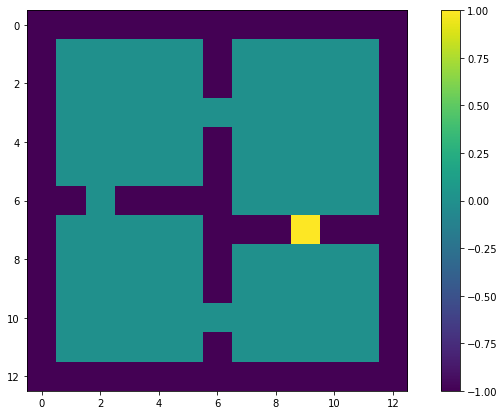
\includegraphics[width=1\linewidth]{env1.png}
  \captionof{figure}{$Goal_1$ Environment}
  %\label{fig:test1}
\end{minipage}%
\begin{minipage}{.5\textwidth}
  \centering
  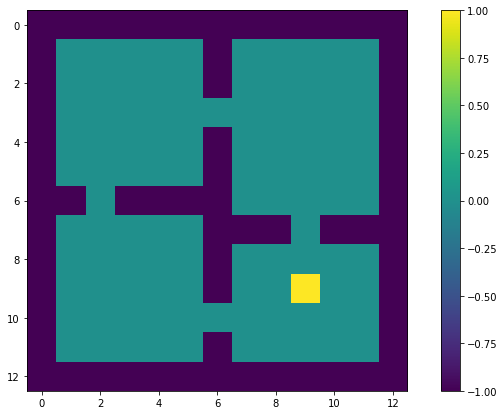
\includegraphics[width=1\linewidth]{env2.png}
  \captionof{figure}{$Goal_2$ Environment}
  %\label{fig:test2}
\end{minipage}
\end{figure}

\item Visualization of learned Q values for start (1,1).
\begin{figure}[htbp!]
\centering
\begin{minipage}{.5\textwidth}
  \centering
  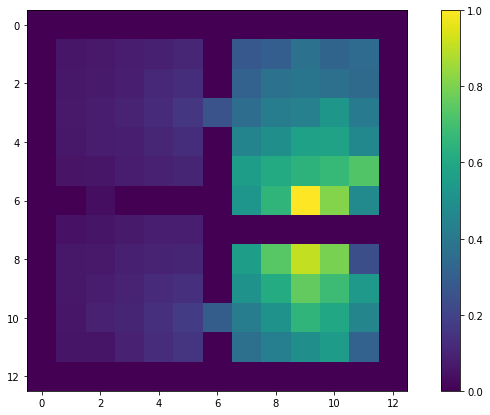
\includegraphics[width=1\linewidth]{1179.png}
  \captionof{figure}{learned value for $goal_1$}
  %\label{fig:test1}
\end{minipage}%
\begin{minipage}{.5\textwidth}
  \centering
  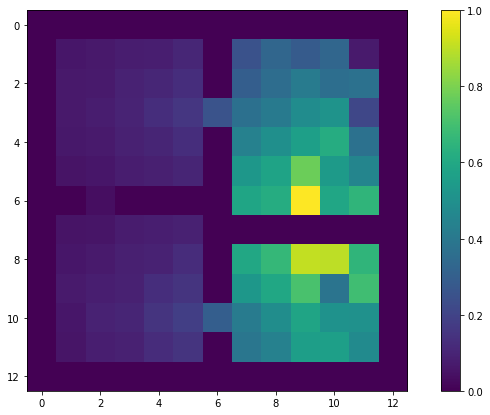
\includegraphics[width=1\linewidth]{1199.png}
  \captionof{figure}{learned value for $goal_2$}
  %\label{fig:test2}
\end{minipage}
\end{figure}


\item Visualization of learned Q values for start centre of 4th room (9,3).
\begin{figure}[htbp!]
\centering
\begin{minipage}{.5\textwidth}
  \centering
  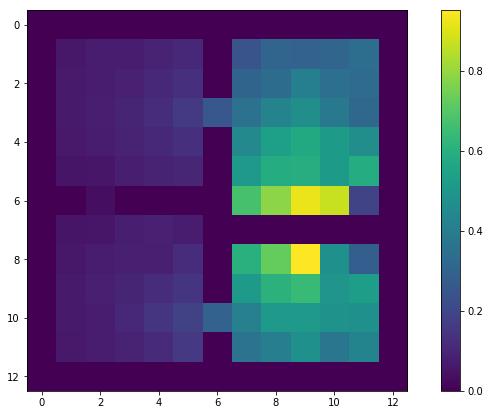
\includegraphics[width=1\linewidth]{9379.png}
  \captionof{figure}{learned value for $goal_1$}
  %\label{fig:test1}
\end{minipage}%
\begin{minipage}{.5\textwidth}
  \centering
  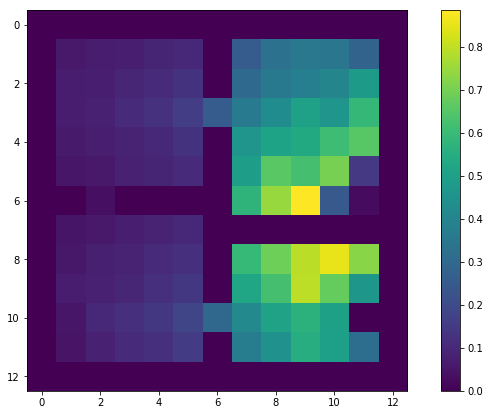
\includegraphics[width=1\linewidth]{9399.png}
  \captionof{figure}{learned value for $goal_2$}
  %\label{fig:test2}
\end{minipage}
\end{figure}
\item On implementing Intra options Q learning , We observe improvement because for a particular option also we get optimal policy.

\end{itemize}

\newpage
\section*{Solution: 2}
Deep Q-Learning solution of CartPole problem.
\begin{itemize}
\item DQN: Q-Learning but with a Deep Neural Network as a function approximator.
Using a non-linear Deep Neural Network is powerful, but training is unstable if we apply it naively.
\item Trick 1 - Experience Replay: Store experience $(S, A, R, S_next)$ in a replay buffer and sample minibatches from it to train the network. This decorrelates the data and leads to better data efficiency. In the beginning, the replay buffer is filled with random experience.
\item Trick 2 - Target Network: Use a separate network to estimate the TD target. This target network has the same architecture as the function approximator but with frozen parameters. Every T steps (a hyperparameter) the parameters from the Q network are copied to the target network. This leads to more stable training because it keeps the target function fixed (for a while).
\end{itemize}
\begin{figure}[htbp!]
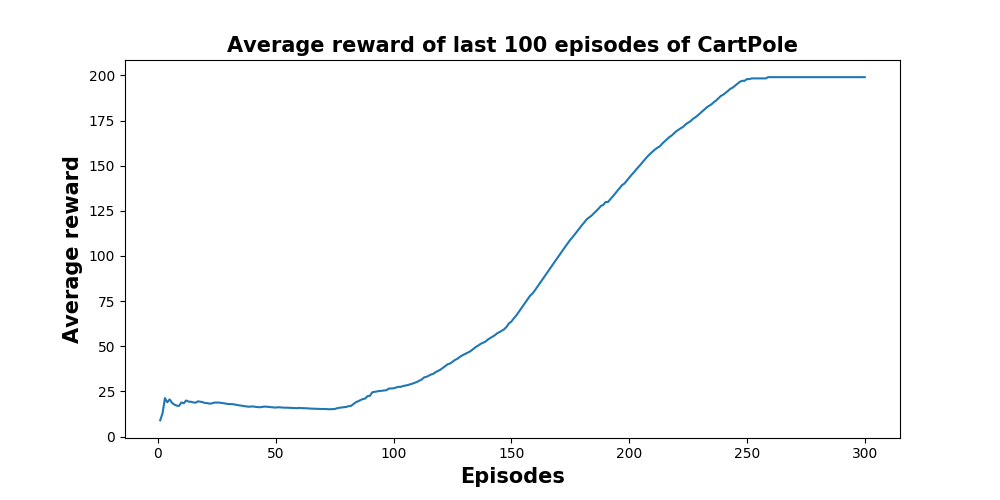
\includegraphics[scale=0.6]{average_reward.png}
\caption{Training Episodes of CartPole with DQN (Experience replay and Target network) }
\end{figure}
\begin{itemize}
\item The problem is solved, As above we can see the average reward for past 100 episodes is around 195 in 260 training episodes.
\item Hyperparameters that work best for me are :  
\begin{itemize}
\item Replay memory size = $1000$
\item Epsilon = $1$
\item Epsilon decay time = $100$
\item Epsilon decay rate = $0.9$
\item Hidden $layer_1$ size =$128$
\item Hidden $layer_2$ size =$128$
\item Hidden $layer_3$ size =$128$
\item Max episodes = 400
\item Max steps = 200
\item Learning rate = 0.001
\item Discount factor = 0.95
\item Minibatch size = 200
\item target update frequency = 100
\end{itemize}
\item Agent learn faster on below given  variation of hyperparameters:
\begin{itemize}
\item On increasing number of hidden layer and its size, the agent learn faster.
\item Epsilon decay rate close to 0.9 make better learning.
\item Replay memory size too low, have low learning.
\item On increasing minibatch size agent learn faster. 
\end{itemize}

\item On removing Experience Replay and target network learning become too slow , and agent average reward is only 100 for 300 episodes.
\begin{figure}[htbp!]
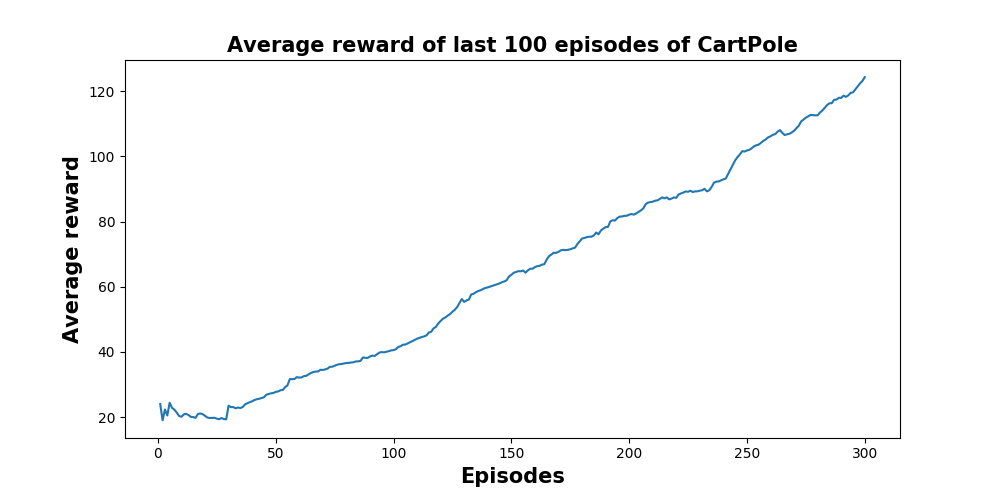
\includegraphics[scale=0.6]{average_reward2.png}
\caption{Training Episodes of CartPole without Experience replay. }
\end{figure}
\end{itemize}

\newpage 

\end{document}